\documentclass[11pt]{article}
\usepackage[margin=1in]{geometry}
\usepackage{setspace}
\usepackage[authoryear,round]{natbib}
\usepackage{booktabs,amsmath,amssymb,graphicx,microtype,hyperref}
\hypersetup{pdftitle={Surface Ties and Stereotype Updating Across Language Model Readouts},pdfauthor={An-Sheng Jhang},colorlinks=true,linkcolor=blue,citecolor=blue,urlcolor=blue}
\onehalfspacing
\raggedbottom
\setlength{\emergencystretch}{3em}
\title{Surface Ties and Stereotype Updating Across Language Model Readouts: A Multi-Channel Measurement Study}
\author{An-Sheng Jhang\\Dongguan University of Technology\\\texttt{ansheng.jhang@gmail.com}}
\date{November 2026\\Working paper}
\begin{document}
\maketitle
\begin{abstract}
Formal tests on these templates detect no directional differences, yet whether the same items appear tied depends on the readout: a surface tie cannot establish absence of bias. We analyze 44,640 records from 11 cohorts and 96 templates. Across 1,012 confirmatory components, zero directional tests survive Holm correction; seven support local equivalence within $\pm0.20$ logit, not exact zero. RQ1/F3 is unavailable without verified human norms. Retaining each model/stance's Direct-100 baseline-tie denominator, MCW-100 breaks 63.51\%--98.57\% of ties (96 templates, six models; broken-subset cell means 4.03--18.91 percentage points), numeric-token readouts break 93.33\%--100.00\% (96 templates, two OpenAI models; 3.36--4.81 points), and Direct-13 breaks 0.00\%--45.45\% (24-template intersection, three models; nonempty means 7.69--46.15 points). All 16 percentage-scale target cells exhibit both positive and negative item displacements; 22/22 signed-mean intervals include zero and 19/22 strictly cross it. These are static descriptions, not explanations for nonsignificant dynamic tests. Exploratory stratification shows MCW-100 yields smaller mean absolute gaps than Direct-100 in 11/11 estimable baseline-nontie cells while breaking ties elsewhere. Scale compression shows heterogeneous halfwidth ratios across models. Alignment and belief-state mechanisms remain unverified hypotheses. Code and data are planned for release at \url{https://github.com/asj252/llm-judgment-studies}, with a Hugging Face dataset to follow; neither is publicly released yet. AI assistance from Antigravity/Gemini, OpenAI Codex CLI, and Claude CLI supported research workflows, coding, drafting or review; the human author verified the manuscript and retains full responsibility for all content.
\end{abstract}
\noindent\textbf{Keywords:} Social cognition; Stereotype updating; Individuating evidence; Psychometrics; Attribution stance; Large language models; Multi-channel measurement

\section{Introduction}
An equal pair of answers is easy to overinterpret. If a language model assigns the same probability to matched social targets, the equality may be read as evidence of unbiased judgment. That interpretation requires a measurement assumption: the equality must be stable across defensible ways of asking and reading the response. This study tests that assumption while separately examining how models update judgments after individuating evidence.

Our main claim is deliberately restricted. On this set of templates, formal tests do not establish directional differences in updating, but item-level equality changes with the readout. We distinguish three units throughout: an individual template pair, a model-by-stance cell mean, and a confirmatory test component. A sizable mean gap among broken ties is not a gap shared by every item. A nonsignificant updating contrast does not establish fairness, and a local equivalence test does not establish exact equality.

The design combines paired social templates, two attribution instructions, controlled weakening evidence, and several numeric readouts. Its contribution is a measurement comparison rather than a new fairness benchmark with an externally validated ground truth. A conditional descriptive pattern is that the same MCW readout that breaks many baseline ties reduces average absolute differences among baseline nonties. Thus a single unconditional claim that this readout increases or decreases gaps would discard information needed to understand its behavior.

\section{Theoretical Background and Related Work}
Social judgments can combine categorical expectations with individuating information. The stereotype content model motivates separate warmth and competence dimensions \citep{fiske2002_scm}, while the continuum account describes the relation between category-based and individuating impressions \citep{fiske1990_individuation_continuum}. Disconfirming cases can be treated as exceptional subtypes rather than revising a category \citep{kunda1995_subtyping}. These theories motivate controlled contrasts here; they do not establish that a language model implements the corresponding human processes.

Cultural knowledge and personal endorsement are conceptually separable \citep{devine1989_cultural_vs_personal}. We therefore contrast Model-Endorsed judgments with Bystander-Predicted judgments. Work on perspective elicitation and social desirability already motivates such distinctions \citep{chapala2025_sdb_perspective_collision}; we make no priority claim for third-person questioning. Neither instruction gives access to a private belief state. Evidence of biased associations despite explicitly unbiased answers \citep{bai2025_implicit_bias} and discrimination in model decisions \citep{tamkin2023_discrim_eval} further cautions against equating an answer surface with a validated fairness property. BBQ studies bias under differing information conditions \citep{parrish2022_bbq}; our focus is paired continuous readouts and subsequent updating rather than benchmark accuracy.

Defeasible inference provides a way to specify evidence that weakens an initially plausible conclusion \citep{rudinger2020thinking}. Graded inference \citep{chen2020uncertain} and belief revision research \citep{wilie2024belief} motivate separating uncertainty from categorical conclusions. We operationalize updating on a clipped logit scale and include neutral and trait-swapped controls so that ordinary response changes need not be attributed to category-specific effects.

Elicitation is itself a measurement choice. Confidence-elicitation evaluations \citep{xiong2024llms} and calibrated verbal confidence strategies \citep{tian2023just} motivate examining how response formats affect numerical outputs. Verbalized Sampling addresses diversity in generation \citep{verbalized_sampling_core}; our weighted multi-candidate readout adapts the general idea of eliciting alternatives to a constrained probability judgment, without importing claims about open-ended diversity or calibration. Scored-versus-generated comparisons in a retail setting \citep{scored_vs_generated2026_readouts} motivate a readout contrast, without demonstrating its validity for social judgments.

Two recent measurement examples broaden this caution. The version-one negation-bias replication \citep{allar2026_negation} places linguistic formulation within the scope of model-based social measurement. The version-one bookmark-style difficulty framework \citep{han2026_bookmark} concerns placement-based item difficulty prediction. Neither evaluates our paired stereotype-updating design. Together they motivate treating wording, scale and elicitation as explicit measurement conditions rather than interchangeable interfaces.

\section{Method and Pre-Collection Internally Frozen Design}
\subsection{Templates, arms and attribution instructions}
The formal design contains 96 synthetic templates, divided across warmth (W) and competence (C). Occupation (O), gender (G), and race-by-gender (R) are separate sensitivity strata; they are not a fully crossed occupation-by-gender-by-race factorial design. Neutral (N) controls support comparison with social targets. A registered 24-template intersection supports the smaller-scale comparison, with 12 templates per dimension. Registration here refers to an internal pre-collection design record, not public OSF preregistration.

Each template has five arms. A is the stereotype target, B the reverse/control prior comparison, C1 a neutral stereotype-trait control, D the trait-swapped target, and C2 a neutral swapped-trait control. The prior state is $P_0$; weakening evidence produces the post-evidence state $P_1$. The collected evidence conditions and control arms follow the frozen stimulus specification. Calls are independent, without conversational memory between items. The two attribution instructions are Model-Endorsed (the archived subjective condition) and Bystander-Predicted (the archived observer condition). The latter asks for a prediction about an observer, not a verified measure of population opinion.

For example, FRM-01 places a person near a community-garden tool shed. A asks whether a pediatric nurse is ``warm and helpful''; B asks the same of a corporate investment banker; C1 asks it of a local resident. D asks whether the nurse is ``cold and uncaring'', and C2 asks the latter of a local resident. The warmth claim is weakened by letting a heavy gate slam shut in front of a parent with two bulky strollers; the coldness claim is weakened by holding the gate open for that parent. The prior prompt presents the scene and statement, and the update prompt adds the corresponding evidence before eliciting the probability again.

Six models supply percentage-scale verbal cohorts: Qwen3-8B, Spark-X2.6, Nemotron-120B, Gemini-3.8-Flash, GPT-4.1-mini and GPT-4.1. The two OpenAI models additionally supply same-model numeric-token cohorts. GPT-4.1-mini, Gemini and Nemotron supply the registered smaller-scale cohorts. Model names identify the evaluated provider endpoints; the study does not randomly sample a population of models.

\subsection{Readouts and numerical diagnostics}
Direct-100 elicits one percentage. MCW-100 elicits five candidate estimates and self-reported weights; their normalized weighted mean is the reported MCW probability. MCW belongs to the multi-candidate verbalization (MCV) family. Equal-weight means, highest-weight candidates and weighted/unweighted dispersion are retained by the shared parser, but the principal weighted readout here is MCW. Direct-13 elicits an integer on the $0..13$ grid and divides by 13. MCW-13 elicits five integer candidates $z_i\in\{0,\ldots,13\}$ and self-reported nonnegative weights $w_i$. Candidates map to $z_i/13\in[0,1]$, and their normalized weighted mean is $\sum_iw_i(z_i/13)/\sum_iw_i$, with a positive weight sum. Values share a common probability scale. Collection used temperature = 0.0; numeric-token calls requested top\_logprobs = 20.

For \texttt{logprob\_pct}, consider the returned numeric-token candidates $\mathcal K$ at the first numeric-token position after the Probability field. Whitespace and a trailing percent sign are stripped; candidates require a finite log probability and a numeric value $v_k\in[0,100]$. An estimate index or candidate weight is not a probability-field token. Define
\begin{align}
 p_k&=\exp(\ell_k), &m_{\text{num}}&=\sum_{k\in\mathcal K}p_k, &q_k&=p_k/m_{\text{num}},\\
 \hat v_{\text{LP}}&=\sum_{k\in\mathcal K}q_kv_k, &p_{\text{LP}}&=\min(0.99,\max(0.01,\hat v_{\text{LP}}/100)).
\end{align}
Validity requires the strict Probability format and $m_{\text{num}}\ge0.80$. This is an expected numeric value, not a modal token. The associated diagnostic is
\begin{equation}
 H_{\text{num}}=-\sum_{k\in\mathcal K}q_k\log_2q_k.
\end{equation}
It is the entropy of the returned first numeric-token candidates, not full-vocabulary entropy or independently calibrated confidence. Empty numeric mass makes both expectation and entropy undefined. Returned probability mass is provider-approximated and may marginally exceed one before renormalization.

\subsection{Updating contrasts and confirmatory inference}
RQ2 asks whether weakening evidence causes unequal retraction of stereotype-consistent and counter-stereotypic statements relative to neutral controls, or symmetric attenuation of both. Less retraction of the stereotype-consistent statement indicates persistence in that direction; tests also allow the reverse direction.

Probabilities are clipped to $[0.01,0.99]$ for logits. Define retraction as $r=\operatorname{logit}(P_0)-\operatorname{logit}(P_1)$ and let $x=r_A-r_{C1}$ and $y=r_D-r_{C2}$. Then
\begin{equation}
 \Delta\Delta_{\text{logit}}=x-y,\qquad \bar\Delta_{\text{att}}=(x+y)/2.
\end{equation}
The first contrast captures asymmetry; the second retains same-direction changes that can cancel in the first. This algebra prevents interpreting a vanishing difference alone as evidence that both controlled changes vanish.

The internally frozen confirmatory families concern updating asymmetry (F1), readout dissociation with neutral-control conditions (F2), symmetric attenuation (F4), and attribution-stance differences with neutral controls (F5). F5 includes static neutral-prior components as well as updating components. RQ1/F3 = NA because verified human normative baselines were unavailable. We do not replace them with model-generated norms.

Inference uses paired templates, studentized bootstrap intervals with $B=4000$ and seed 20261115, and the frozen Holm correction scheme within its specified cohort/family testing structure. The local equivalence band is $\pm0.20$ logit. A reported significant component must be distinguished from a complete conjunctive family verdict. Missing probabilities exclude the affected pair, with design and observed denominators retained. Undefined studentized replicates and nonestimable quantities follow the frozen rules and remain NA, never numerical zero; the appendix reports missingness and undefined-replicate counts for significant components.

\subsection{Descriptive analyses and provenance}
The frozen \texttt{mid50} statistic is the proportion of valid probabilities in 48\%--52\%, inclusive, equivalently $|p-0.50|\le0.02$. It pools the valid readouts in each archived cohort: Direct and MCW for verbal cohorts and the numeric-token readout for numeric-token cohorts. On the smaller scale only the weighted MCW output can enter this band.

A static surface tie is $|P_A-P_B|\le10^{-12}$ at $P_0$ in Direct-100. Tie-breaking rates use the original tied-pair denominator, retaining missing target pairs in that denominator but excluding them from broken counts and magnitude summaries. Broken-subset absolute cell means and valid-subset signed means answer different questions. Differences in this analysis are percentage points (pp), with signed direction A minus B. The locked tie-summary intervals use a percentile bootstrap with replacement. They are descriptive, without a new confirmatory test or multiplicity claim.

The additional all-template and nontie summaries are explicitly exploratory. Their bootstrap sorts by template identifier and draws indices with a fresh seeded generator per cell; samples remain paired within templates. They retain all valid P0 pairs or stratify by the original Direct-100 nontie status. All outputs preserve source hashes. The internal SHA-256 freeze predates formal collection and binds stimuli, prompts, collection and evaluation code, seed and resampling count. It is not a public timestamped preregistration. Development records are excluded from every formal analysis.

\section{Results}
\subsection{Compliance, Refusal Rates, and Scale-100 Midpoint Proximity}
[Descriptive / Exploratory] Compliance totals were 44,640 records in 11 cohorts, with 44,629 valid probabilities and 0 refusals (0.00\%); 11 probabilities were invalid, all in Qwen3-8B. No refusal does not establish unbiased responses. Table~\ref{tab:cohorts} separates cohort record counts from valid probabilities.

The frozen \texttt{mid50} statistic is the proportion of valid probabilities in 48\%--52\%, inclusive, equivalently $|p-0.50|\le0.02$. It pools the valid readouts in each archived cohort: Direct and MCW for verbal cohorts and the numeric-token readout for numeric-token cohorts. On the smaller scale only the weighted MCW output can enter this band.

[Descriptive / Exploratory] R midpoint proximity was highest in 4/6 percentage-scale verbal cohorts. The statistic concerns proximity to 50\% on that scale rather than a test of social bias, and its denominator is valid probabilities. Figure~\ref{fig:4} and Tables~\ref{tab:mid0} and \ref{tab:mid1} retain all strata and cohorts.
For Qwen3-8B, midpoint proximity was R 16.58\%, O 18.90\%, N 18.02\%. R is below both listed comparison strata.
For Spark-X2.6, midpoint proximity was R 8.51\%, O 8.59\%, N 9.03\%. R is below both listed comparison strata.

\begin{figure}[p]\centering
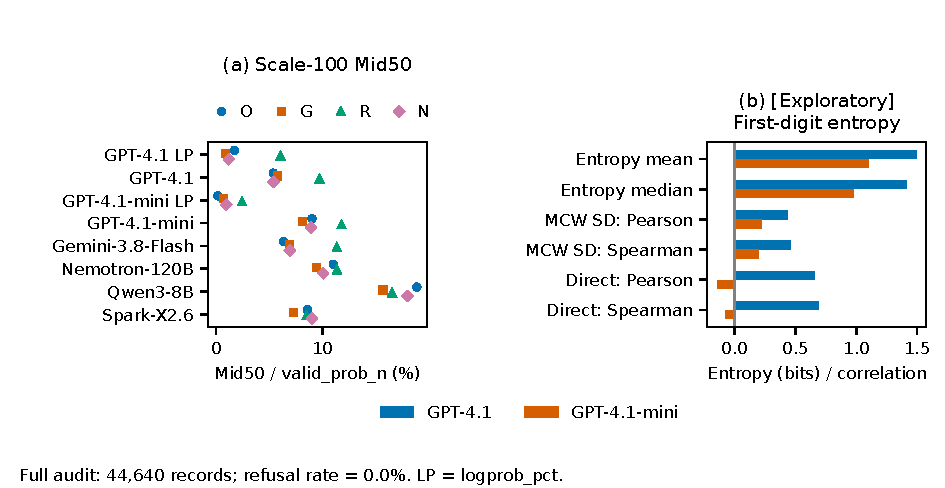
\includegraphics[width=\textwidth,height=.65\textheight,keepaspectratio]{figures/fig4_mid50_and_entropy.pdf}
\caption{[Descriptive / Exploratory] Midpoint proximity by stratum and numeric diagnostics. The figure's first-digit entropy shorthand denotes first numeric-token candidate entropy, not full-vocabulary entropy.}\label{fig:4}
\end{figure}

\subsection{Aggregate Static Baselines and Confirmatory Updating Tests}
[Descriptive / Exploratory] The P0 Model-Endorsed three-channel range was $-1.36$ to $+1.77$ pp across Direct-100, MCW-100 and \texttt{logprob\_pct}, using 96 templates and 14 model-by-readout cells.
The P0 Model-Endorsed four-channel range was $-1.36$ to $+8.33$ pp across 17 cells, including Direct-13 on its 24-template intersection.
The P0 both-stance three-channel range was $-3.15$ to $+2.98$ pp across 28 cells using the 96-template channels.
The P0 both-stance four-channel range was $-3.15$ to $+8.33$ pp across 34 cells including the smaller intersection. These are ranges of signed cell means over all available templates, not ranges of individual item effects.

[Confirmatory] Family component results were F1: 0/264; F2: 0/132; F4: 3/264; F5: 4/352; total 7/1,012. Directional significance: 0. All significant components test local equivalence within $\pm0.20$ logit. Tables~\ref{tab:families}, \ref{tab:sig}, and \ref{tab:effects} give denominators, component identities and estimates; Figure~\ref{fig:2} places asymmetry and attenuation intervals on their analysis scale.
For Gemini-3.8-Flash verbal F4 Model-Endorsed Warmth MCW, the estimate was $-0.0121$ logit, CI $[-0.0877,0.0651]$ logit, and adjusted $p=0.0060$.
For GPT-4.1 numeric-token F5 Competence N-prior, the estimate was $0.0111$ logit, CI $[-0.0898,0.1140]$ logit, and adjusted $p=0.0240$.
For GPT-4.1-mini numeric-token F4 Model-Endorsed Warmth Direct, the estimate was $0.0600$ logit, CI $[-0.0157,0.1455]$ logit, and adjusted $p=0.0172$.
For GPT-4.1-mini numeric-token F4 Bystander-Predicted Warmth Direct, the estimate was $0.0046$ logit, CI $[-0.0802,0.0804]$ logit, and adjusted $p=0.0060$.
For GPT-4.1-mini numeric-token F5 Warmth N-prior, the estimate was $0.0133$ logit, CI $[-0.0531,0.0866]$ logit, and adjusted $p=0.0080$.
For GPT-4.1-mini numeric-token F5 Warmth N-update, the estimate was $-0.0368$ logit, CI $[-0.1192,0.0568]$ logit, and adjusted $p=0.0080$.
For GPT-4.1-mini numeric-token F5 Competence N-prior, the estimate was $-0.0301$ logit, CI $[-0.1107,0.0486]$ logit, and adjusted $p=0.0080$.

Each of these components uses 48/48 pairs with no missing pairs or undefined bootstrap replicates. Three of the four F5 components concern static N-prior contrasts. They are neutral-control results, not evidence that the full attribution family is equivalent. Likewise, the three F4 components do not characterize every model, dimension or readout. Equivalence within the tolerance band is not exact zero; an Inconclusive verdict is not absence of bias. The results support neither a universal updating failure nor a universal absence of updating asymmetry.

\begin{figure}[p]\centering
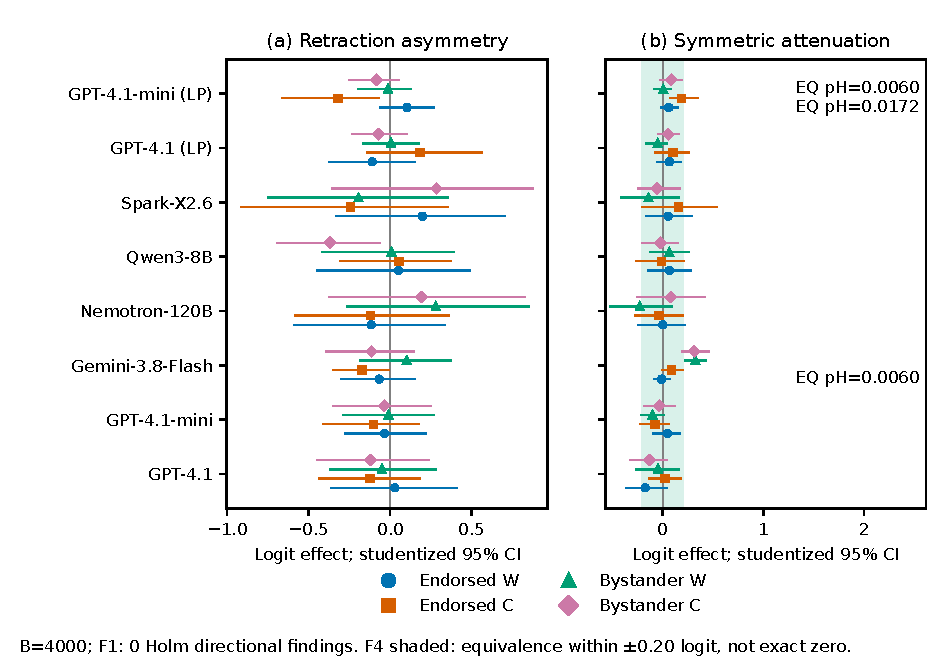
\includegraphics[width=\textwidth,height=.65\textheight,keepaspectratio]{figures/fig2_rq2_forest.pdf}
\caption{[Confirmatory] Frozen F1 asymmetry and F4 symmetric attenuation contrasts with studentized intervals. Verbal cohorts show MCW; numeric-token cohorts show Direct. The equivalence band permits nonzero effects.}\label{fig:2}
\end{figure}

\subsection{Item-Level Surface Ties, Tie-Breaking Magnitudes, Directional Distributions, and Non-Tie Stratification}
[Descriptive / Exploratory] For the MCW-100 tie comparison, we observed a design of 96 templates and 6 models; tie-breaking rates 63.51\%--98.57\%; broken-subset absolute cell means 4.03--18.91 pp.
For the Numeric-token logprob\_pct tie comparison, we observed a design of 96 templates and 2 OpenAI models; tie-breaking rates 93.33\%--100.00\%; broken-subset absolute cell means 3.36--4.81 pp.
For the Direct-13 tie comparison, we observed a design of 24 templates and 3 models; tie-breaking rates 0.00\%--45.45\%; nonempty broken-subset absolute cell means 7.69--46.15 pp.

These are design coverage sizes, not the actual baseline-tie denominators. Table~\ref{tab:ties} and Figure~\ref{fig:1} report the original integer counts. The magnitude ranges are ranges of model-by-stance means within the broken subsets, not per-item minimum and maximum displacements. Tables~\ref{tab:delta_MCW100}, \ref{tab:delta_Direct13}, and \ref{tab:delta_logprobpct} retain signed means separately from absolute magnitudes.

For Qwen3-8B, each stance has 1 missing target pair. Its Model-Endorsed comparison is 49/77, with 76 valid target pairs; its Bystander-Predicted comparison is 47/74, with 73 valid target pairs. The missing pair enters neither the broken numerator nor difference summaries; the baseline-tie denominator is retained.
For Nemotron-120B Bystander-Predicted Direct-13, the observed tie-breaking rate of 0/24 = 0.00\% is valid. Only the empty broken-subset magnitude is NA; it must not be replaced by a measured zero magnitude.
The signed tie-displacement distribution shows that all 16 percentage-scale target cells contain positive and negative item displacements; 22/22 signed-mean percentile intervals include zero and 19/22 strictly cross zero. The exceptions to strict crossing are the three Direct-13 cells described below.

Nemotron Bystander-Predicted has a degenerate zero interval. GPT-4.1-mini has only negative nonzero displacements in Model-Endorsed and only positive nonzero displacements in Bystander-Predicted; both intervals touch zero. These static patterns neither rule out systematic average shifts nor explain why the separate dynamic confirmatory tests did not establish directional effects.

[Descriptive / Exploratory] For MCW-100 nontie stratification, 11/11 estimable cells have smaller mean absolute gaps, out of 12 cells with 1 empty cell.
For MCW-100 Model-Endorsed nonties, mean absolute gaps span 17.31--46.70 pp under Direct-100 and 10.04--16.58 pp under MCW-100.
Across both stances, MCW-100 nontie mean absolute gaps span 15.80--50.00 pp under Direct-100 and 8.09--19.40 pp under MCW-100.

All 4/4 estimable \texttt{logprob\_pct} nontie cells have smaller mean absolute gaps. Direct-13 has smaller means in 4/5 estimable cells, but GPT-4.1-mini Model-Endorsed increases from 22.22 to 28.21 pp (paired difference +5.98 pp, percentile CI $[-9.91,22.01]$ pp), with 5 shrunk and 4 expanded pairs. Other Direct-13 shrunk/expanded counts are 9/1 for GPT-4.1-mini Bystander-Predicted, 10/4 and 10/3 for Gemini Model-Endorsed and Bystander-Predicted, and 4/0 for Nemotron Model-Endorsed; Nemotron Bystander-Predicted has no eligible nonties. These counts describe pairs rather than cell means. GPT-4.1 Bystander-Predicted MCW-100 has 31 shrunk, 24 expanded and 1 unchanged pair despite its smaller cell mean; the numeric-token comparison has 41 shrunk and 15 expanded. Baseline absolute-gap medians are 50 pp in Qwen, Spark and the estimable Nemotron MCW cells, with zero interquartile range except Qwen Model-Endorsed (30 pp). This concentration at a coarse response mode limits interpretation of contraction beyond the conditional descriptive comparison.

The endpoints need not arise from the same cells. The all-cell paired comparisons, rather than a pairing of range endpoints, establish the descriptive decrease. Stratifying on a baseline measure can induce regression-to-the-mean patterns, especially when exact grid equality defines one stratum. A broken tie equally cannot establish presence of bias. This result therefore rebuts monotonic gap amplification within this dataset; it does not establish general smoothing, debiasing, or a latent causal mechanism.

\begin{figure}[p]\centering
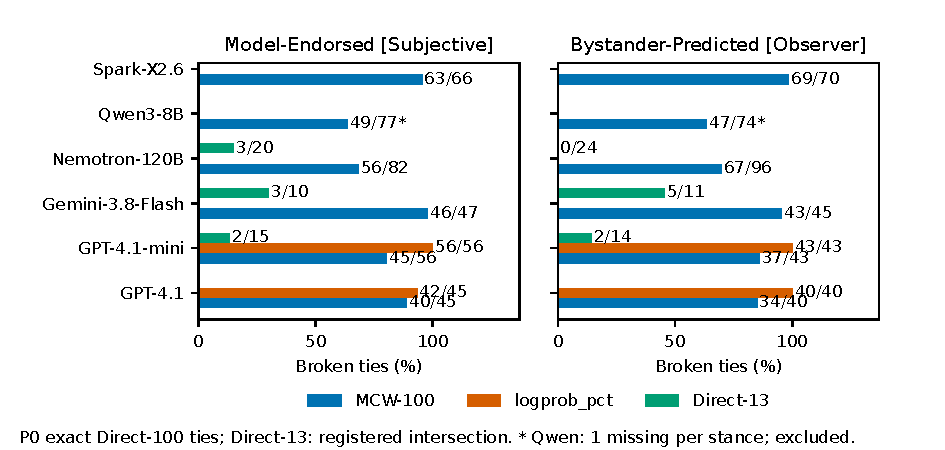
\includegraphics[width=\textwidth,height=.65\textheight,keepaspectratio]{figures/fig1_tie_breaking.pdf}
\caption{[Descriptive / Exploratory] Direct-100 surface ties broken by alternative readouts. Counts retain the original baseline-tie denominator. Direct-13 uses the registered intersection; Qwen missing targets are excluded from broken counts.}\label{fig:1}
\end{figure}

\subsection{Scale Compression (0..13 vs. 0..100) and Numeric-Token Entropy Diagnostics}
[Descriptive / Exploratory] The halfwidth comparison covered F1 / Model-Endorsed / Warmth / 12 pairs per cell. The reported ratio divides the studentized interval halfwidth on the smaller scale by its matched percentage-scale halfwidth; it is not a global ratio across all families or templates (Table~\ref{tab:scale}; Figure~\ref{fig:3}).
The Gemini-3.8-Flash halfwidth MCW ratio was 1.0470x.
The Gemini-3.8-Flash halfwidth Direct ratio was 0.9295x.
The Nemotron-120B halfwidth MCW ratio was 0.7155x.
The Nemotron-120B halfwidth Direct ratio was 1.0904x.
The GPT-4.1-mini halfwidth MCW ratio was 1.5858x.
The GPT-4.1-mini halfwidth Direct ratio was 2.6819x.

Both GPT-4.1-mini ratios exceed one; only Nemotron and Gemini have opposite directions across readouts in this matched comparison. Direct prior tie rates did not decrease. Calibration was not assessed because no ground-truth benchmark was available. These differences cannot be attributed to removing the midpoint. A single integer candidate on $0..13$ cannot equal 0.50 after division by 13, but the weighted MCW-13 output can equal exactly 0.50: the archive contains 1 record exactly at 0.50 and 34 records within 48\%--52\%, inclusive. In Table~\ref{tab:scale}, prior tie-rate entries alongside both Direct and MCW rows refer exclusively to Direct readouts, not MCW tie rates.

Numeric-token diagnostics are restricted to the two OpenAI models (Table~\ref{tab:entropy}). Each has adequate numeric mass in every collected numeric-token record. Entropy associations with MCW dispersion are positive, whereas associations with Direct differ by model. These correlations concern paired outputs under the observed prompts; they do not identify a causal relationship or validate the entropy as a confidence score. In particular, $H_{\text{num}}$ is first numeric-token candidate entropy, not the entropy over all possible generated answers.

\begin{figure}[p]\centering
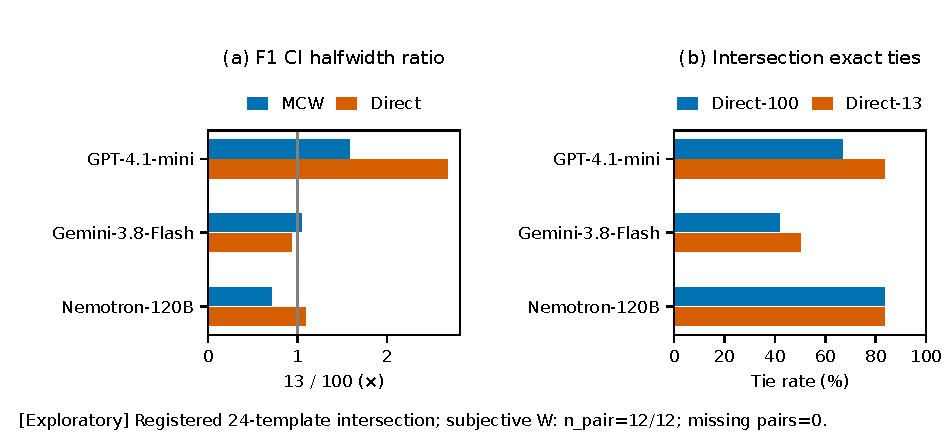
\includegraphics[width=\textwidth,height=.65\textheight,keepaspectratio]{figures/fig3_scale13_heterogeneity.pdf}
\caption{[Descriptive / Exploratory] Registered-intersection scale comparison restricted to Model-Endorsed warmth. Readout-specific halfwidth ratios vary across models; a narrower interval does not establish calibration.}\label{fig:3}
\end{figure}

\section{Discussion, Limitations, and Future Directions}
The central practical implication is to report the readout with the result. A surface tie is a property of a specified response channel and prompt, not an externally validated declaration of fairness. The coexistence of tie breaking and nontie contraction makes stratified reporting particularly useful: investigators should preserve baseline status, signed differences, absolute magnitudes, missingness and design coverage rather than summarize a readout with a single directional slogan.

The confirmatory and descriptive conclusions have different evidential roles. No directional component survives the frozen multiplicity procedure. Seven local equivalence components constrain a limited set of contrasts. Neither result licenses a population-wide assertion that models are unbiased. Static displacement intervals and dynamic updating contrasts also address different quantities, so the former cannot explain the latter merely because both involve differences of probabilities.

\textbf{Unverified hypothesis:} safety alignment or social desirability could affect expressed probabilities. We have no unaligned base-model control, so this study cannot attribute the observed patterns to reinforcement learning from human feedback, suppression, or compensatory alignment. \textbf{Unverified hypothesis:} coarse integer grids could contribute to ties. The smaller-scale comparison is consistent with heterogeneous measurement effects, but it does not isolate grid resolution from instruction interpretation. \textbf{Unverified hypothesis:} a distinction between surface expression and internal belief could produce channel differences. Our data do not measure private beliefs; generated estimates and returned token probabilities are both behavior under an elicitation protocol.

Several limitations follow. Synthetic English templates have limited ecological and linguistic coverage. The stimuli and six principal models are purposive rather than representative samples. The small-scale intersection contains fewer templates, and numeric-token diagnostics cover only two OpenAI models. Provider approximation and truncation affect the candidate distribution. MCW weights are self-reported and need not represent independent samples or calibrated probabilities. Missing outputs and degenerate studentization require explicit NA handling. Multiple testing reduces power; lack of significance can coexist with substantial uncertainty. The added nontie stratification was not a preregistered confirmatory hypothesis and may reflect conditioning on a noisy baseline. Verified human norms, behavioral outcomes and an unaligned model comparison are absent. Internal hashing supports reproducibility but cannot supply the independent timing assurance of public preregistration.

Future studies should separate fixed-weight instruction interventions from controlled training comparisons that change weights. The former can randomize response format, attribution wording and evidence strength within a fixed endpoint. The latter should compare aligned and base checkpoints with documented training differences and matched evaluation conditions before making causal claims about alignment. Repeated measurements and held-out stimuli can assess the stability of baseline strata and distinguish systematic contraction from regression to the mean. Independently validated human norms would permit the presently unavailable normative comparisons. None of these proposed tests has been completed here.

\section{Transparency, Ethics, and Disclosure Statements}
\subsection{Data and Code Availability}
The code and all 44,640 formal data records have been organized and validated locally. Public release is planned alongside publication of this working paper at \url{https://github.com/asj252/llm-judgment-studies}, with a synchronized companion Hugging Face Dataset. The code and data release is not yet publicly available. No external dataset URL is claimed. The analysis uses the archived formal records and excludes development probes.

\subsection{Analytical Freeze and Transparency}
The pre-collection internal freeze records SHA-256 fingerprints and analysis settings. It is not public OSF preregistration, and no public registration link is asserted. Confirmatory and exploratory analyses are labeled separately. Exploratory P0 all-template and nontie analyses were added during manuscript preparation; the original data, tables, figures and evaluation outputs remain locked. Reproducibility checks compare archived-source hashes and independently recomputed summaries, and compile the manuscript outside the repository.

\subsection{Conflict of Interest and Ethics Statement}
The author declares no competing financial or personal interests. This research received no specific external grant funding. Because this study evaluates large language model outputs on controlled synthetic text templates and involves no human participants, animals, or private personal data, institutional ethics review for human-subjects research is not applicable. Sensitive demographic categories are used strictly for measurement, not endorsement of stereotypes or decisions about identifiable individuals.

\subsection{AI and LLM Tool Use Disclosure}
Antigravity/Gemini assisted the project's research workflow, source organization and planning. OpenAI Codex CLI assisted computational implementation, numerical verification, English manuscript drafting and revision, and engineering checks. Claude CLI completed an independent review of this manuscript's structure and readability, retained in the delivery record. The English draft was prepared directly with AI assistance under the author's authorized design decisions; no completed handwritten Chinese manuscript or translation is claimed. The human author conceived the study, directed the design and revisions, verified the claims, citations, computations, figures, and final text, and takes full responsibility for all content. No AI system is listed as an author. Model outputs used as experimental observations are distinct from these research-assistance roles.

\clearpage
\bibliographystyle{plainnat}
\bibliography{references}
\clearpage\appendix
\section{Full Locked Tables}
\subsection*{Scope and interpretation cards}
RQ1/F3 = NA: human normative baselines were unavailable; only RQ2 families F1, F2, F4, F5 are reported.
R midpoint proximity is highest in 4 of 6 percentage-scale verbal cohorts.
Exceptions: Qwen3-8B R 16.58\% $<$ O 18.90\%, N 18.02\%; Spark-X2.6 R 8.51\% $<$ O 8.59\%, N 9.03\%.
Direct-13: 24 templates, 3 models, 0.00\%--45.45\%; MCW-100: 96 templates, 6 models, 63.51\%--98.57\%; logprob\_pct: 96 templates, 2 OpenAI models, 93.33\%--100.00\%.
These design sizes differ; rates retain each model/stance's baseline-tie denominator.
Holm significant/total: F1: 0/264; F2: 0/132; F4: 3/264; F5: 4/352; total 7/1,012.
All 7 significant components are p\_EQ equivalence tests; directional significance: 0.
Halfwidth ratios concern only F1 / Model-Endorsed / Warmth / 12 pairs per cell.
GPT-4.1-mini MCW 1.5858x and Direct 2.6819x are both $>$ 1; opposite readout directions occur only for Nemotron and Gemini.
Tie deltas are descriptive percentage points (pp), Arm A - Arm B, with no new confirmatory tests.

% TABLE cohorts
\begin{table}[htbp]\centering\small
\setlength{\tabcolsep}{3pt}
\resizebox{\textwidth}{!}{\begin{tabular}{lllllll}
\toprule
Model & Scale & Ch. & Records & Valid & Refused & Refusal \\
\midrule
Qwen3-8B & 100 & V & 5760 & 5749 & 0 & 0.00\% \\
Spark-X2.6 & 100 & V & 5760 & 5760 & 0 & 0.00\% \\
Nemotron-120B & 100 & V & 5760 & 5760 & 0 & 0.00\% \\
Gemini-3.8-Flash & 100 & V & 5760 & 5760 & 0 & 0.00\% \\
GPT-4.1-mini & 100 & V & 5760 & 5760 & 0 & 0.00\% \\
GPT-4.1 & 100 & V & 5760 & 5760 & 0 & 0.00\% \\
GPT-4.1-mini & 100 & LP & 2880 & 2880 & 0 & 0.00\% \\
GPT-4.1 & 100 & LP & 2880 & 2880 & 0 & 0.00\% \\
GPT-4.1-mini & 13 & V & 1440 & 1440 & 0 & 0.00\% \\
Gemini-3.8-Flash & 13 & V & 1440 & 1440 & 0 & 0.00\% \\
Nemotron-120B & 13 & V & 1440 & 1440 & 0 & 0.00\% \\
\bottomrule\end{tabular}}
\caption{Record counts, valid probabilities and refusals. V: verbal; LP: same-model logprob readout.}
\label{tab:cohorts}
\end{table}

% TABLE sig
\begin{table}[htbp]\centering\small
\setlength{\tabcolsep}{3pt}
\resizebox{\textwidth}{!}{\begin{tabular}{llllllll}
\toprule
ID & Model & Ch. & Component & Pairs/design & Miss. & Undef. & pH \\
\midrule
1 & Gemini-3.8-Flash & V & F4:E:W:M & 48/48 & 0 & 0 & 0.0060 \\
2 & GPT-4.1 & LP & F5:C:N-prior & 48/48 & 0 & 0 & 0.0240 \\
3 & GPT-4.1-mini & LP & F4:E:W:D & 48/48 & 0 & 0 & 0.0172 \\
4 & GPT-4.1-mini & LP & F4:B:W:D & 48/48 & 0 & 0 & 0.0060 \\
5 & GPT-4.1-mini & LP & F5:W:N-prior & 48/48 & 0 & 0 & 0.0080 \\
6 & GPT-4.1-mini & LP & F5:W:N-update & 48/48 & 0 & 0 & 0.0080 \\
7 & GPT-4.1-mini & LP & F5:C:N-prior & 48/48 & 0 & 0 & 0.0080 \\
\bottomrule\end{tabular}}
\caption{All Holm-significant components. IDs link to the effect table. E/B: endorsed/bystander; W/C: warmth/competence; D/M: Direct/MCW. All are local equivalence components, not full family findings.}
\label{tab:sig}
\end{table}

% TABLE effects
\begin{table}[htbp]\centering\small
\setlength{\tabcolsep}{3pt}
\resizebox{\textwidth}{!}{\begin{tabular}{lllllll}
\toprule
ID & Model & Family & Estimate & CI lower & CI upper & Records \\
\midrule
1 & Gemini-3.8-Flash & F4 & -0.0121 & -0.0877 & 0.0651 & 5760 \\
2 & GPT-4.1 & F5 & 0.0111 & -0.0898 & 0.1140 & 2880 \\
3 & GPT-4.1-mini & F4 & 0.0600 & -0.0157 & 0.1455 & 2880 \\
4 & GPT-4.1-mini & F4 & 0.0046 & -0.0802 & 0.0804 & 2880 \\
5 & GPT-4.1-mini & F5 & 0.0133 & -0.0531 & 0.0866 & 2880 \\
6 & GPT-4.1-mini & F5 & -0.0368 & -0.1192 & 0.0568 & 2880 \\
7 & GPT-4.1-mini & F5 & -0.0301 & -0.1107 & 0.0486 & 2880 \\
\bottomrule\end{tabular}}
\caption{Studentized 95 percent confidence intervals for the component IDs above; equivalence is relative to the frozen logit band, never exact zero.}
\label{tab:effects}
\end{table}

% TABLE ties
\begin{table}[htbp]\centering\small
\setlength{\tabcolsep}{3pt}
\resizebox{\textwidth}{!}{\begin{tabular}{lllllll}
\toprule
Model & Stance & Target & Design & Broken/base & Miss. & Rate \\
\midrule
Gemini-3.8-Flash & E & MCW-100 & 96 & 46/47 & 0 & 97.87\% \\
Gemini-3.8-Flash & E & Direct-13 & 24 & 3/10 & 0 & 30.00\% \\
Gemini-3.8-Flash & B & MCW-100 & 96 & 43/45 & 0 & 95.56\% \\
Gemini-3.8-Flash & B & Direct-13 & 24 & 5/11 & 0 & 45.45\% \\
Nemotron-120B & E & MCW-100 & 96 & 56/82 & 0 & 68.29\% \\
Nemotron-120B & E & Direct-13 & 24 & 3/20 & 0 & 15.00\% \\
Nemotron-120B & B & MCW-100 & 96 & 67/96 & 0 & 69.79\% \\
Nemotron-120B & B & Direct-13 & 24 & 0/24 & 0 & 0.00\% \\
GPT-4.1 & E & MCW-100 & 96 & 40/45 & 0 & 88.89\% \\
GPT-4.1 & E & LP & 96 & 42/45 & 0 & 93.33\% \\
GPT-4.1 & B & MCW-100 & 96 & 34/40 & 0 & 85.00\% \\
GPT-4.1 & B & LP & 96 & 40/40 & 0 & 100.00\% \\
GPT-4.1-mini & E & MCW-100 & 96 & 45/56 & 0 & 80.36\% \\
GPT-4.1-mini & E & Direct-13 & 24 & 2/15 & 0 & 13.33\% \\
GPT-4.1-mini & E & LP & 96 & 56/56 & 0 & 100.00\% \\
GPT-4.1-mini & B & MCW-100 & 96 & 37/43 & 0 & 86.05\% \\
GPT-4.1-mini & B & Direct-13 & 24 & 2/14 & 0 & 14.29\% \\
GPT-4.1-mini & B & LP & 96 & 43/43 & 0 & 100.00\% \\
Qwen3-8B & E & MCW-100 & 96 & 49/77 & 1 & 63.64\% \\
Qwen3-8B & B & MCW-100 & 96 & 47/74 & 1 & 63.51\% \\
Spark-X2.6 & E & MCW-100 & 96 & 63/66 & 0 & 95.45\% \\
Spark-X2.6 & B & MCW-100 & 96 & 69/70 & 0 & 98.57\% \\
\bottomrule\end{tabular}}
\caption{All Direct-100 prior-tie comparisons. Missing target pairs are excluded from broken counts, while the frozen baseline-tie denominator is retained. Qwen has one missing target pair in each stance. Direct-13 uses only the registered intersection.}
\label{tab:ties}
\end{table}

% TABLE mid0
\begin{table}[htbp]\centering\small
\setlength{\tabcolsep}{3pt}
\resizebox{\textwidth}{!}{\begin{tabular}{lllllllll}
\toprule
Model & Scale & Ch. & Str. & Records & Valid & Mid & Rate & Refused \\
\midrule
Qwen3-8B & 100 & V & O & 1152 & 1148 & 217 & 18.90\% & 0 \\
Qwen3-8B & 100 & V & G & 1152 & 1151 & 181 & 15.73\% & 0 \\
Qwen3-8B & 100 & V & R & 1152 & 1152 & 191 & 16.58\% & 0 \\
Qwen3-8B & 100 & V & N & 2304 & 2298 & 414 & 18.02\% & 0 \\
Spark-X2.6 & 100 & V & O & 1152 & 1152 & 99 & 8.59\% & 0 \\
Spark-X2.6 & 100 & V & G & 1152 & 1152 & 84 & 7.29\% & 0 \\
Spark-X2.6 & 100 & V & R & 1152 & 1152 & 98 & 8.51\% & 0 \\
Spark-X2.6 & 100 & V & N & 2304 & 2304 & 208 & 9.03\% & 0 \\
Nemotron-120B & 100 & V & O & 1152 & 1152 & 127 & 11.02\% & 0 \\
Nemotron-120B & 100 & V & G & 1152 & 1152 & 109 & 9.46\% & 0 \\
Nemotron-120B & 100 & V & R & 1152 & 1152 & 131 & 11.37\% & 0 \\
Nemotron-120B & 100 & V & N & 2304 & 2304 & 232 & 10.07\% & 0 \\
Gemini-3.8-Flash & 100 & V & O & 1152 & 1152 & 73 & 6.34\% & 0 \\
Gemini-3.8-Flash & 100 & V & G & 1152 & 1152 & 80 & 6.94\% & 0 \\
Gemini-3.8-Flash & 100 & V & R & 1152 & 1152 & 131 & 11.37\% & 0 \\
Gemini-3.8-Flash & 100 & V & N & 2304 & 2304 & 160 & 6.94\% & 0 \\
GPT-4.1-mini & 100 & V & O & 1152 & 1152 & 104 & 9.03\% & 0 \\
GPT-4.1-mini & 100 & V & G & 1152 & 1152 & 94 & 8.16\% & 0 \\
GPT-4.1-mini & 100 & V & R & 1152 & 1152 & 136 & 11.81\% & 0 \\
GPT-4.1-mini & 100 & V & N & 2304 & 2304 & 206 & 8.94\% & 0 \\
GPT-4.1 & 100 & V & O & 1152 & 1152 & 62 & 5.38\% & 0 \\
GPT-4.1 & 100 & V & G & 1152 & 1152 & 67 & 5.82\% & 0 \\
GPT-4.1 & 100 & V & R & 1152 & 1152 & 112 & 9.72\% & 0 \\
GPT-4.1 & 100 & V & N & 2304 & 2304 & 124 & 5.38\% & 0 \\
\bottomrule\end{tabular}}
\caption{Midpoint proximity by occupation O, gender G, race by gender R and neutral N; rate denominator is valid probabilities. Refusal denominator is all records. Descriptive, not a bias test.}
\label{tab:mid0}
\end{table}

% TABLE mid1
\begin{table}[htbp]\centering\small
\setlength{\tabcolsep}{3pt}
\resizebox{\textwidth}{!}{\begin{tabular}{lllllllll}
\toprule
Model & Scale & Ch. & Str. & Records & Valid & Mid & Rate & Refused \\
\midrule
GPT-4.1-mini & 100 & LP & O & 576 & 576 & 1 & 0.17\% & 0 \\
GPT-4.1-mini & 100 & LP & G & 576 & 576 & 4 & 0.69\% & 0 \\
GPT-4.1-mini & 100 & LP & R & 576 & 576 & 14 & 2.43\% & 0 \\
GPT-4.1-mini & 100 & LP & N & 1152 & 1152 & 11 & 0.95\% & 0 \\
GPT-4.1 & 100 & LP & O & 576 & 576 & 10 & 1.74\% & 0 \\
GPT-4.1 & 100 & LP & G & 576 & 576 & 5 & 0.87\% & 0 \\
GPT-4.1 & 100 & LP & R & 576 & 576 & 35 & 6.08\% & 0 \\
GPT-4.1 & 100 & LP & N & 1152 & 1152 & 14 & 1.22\% & 0 \\
GPT-4.1-mini & 13 & V & O & 288 & 288 & 5 & 1.74\% & 0 \\
GPT-4.1-mini & 13 & V & G & 288 & 288 & 4 & 1.39\% & 0 \\
GPT-4.1-mini & 13 & V & R & 288 & 288 & 2 & 0.69\% & 0 \\
GPT-4.1-mini & 13 & V & N & 576 & 576 & 5 & 0.87\% & 0 \\
Gemini-3.8-Flash & 13 & V & O & 288 & 288 & 2 & 0.69\% & 0 \\
Gemini-3.8-Flash & 13 & V & G & 288 & 288 & 3 & 1.04\% & 0 \\
Gemini-3.8-Flash & 13 & V & R & 288 & 288 & 3 & 1.04\% & 0 \\
Gemini-3.8-Flash & 13 & V & N & 576 & 576 & 8 & 1.39\% & 0 \\
Nemotron-120B & 13 & V & O & 288 & 288 & 1 & 0.35\% & 0 \\
Nemotron-120B & 13 & V & G & 288 & 288 & 0 & 0.00\% & 0 \\
Nemotron-120B & 13 & V & R & 288 & 288 & 1 & 0.35\% & 0 \\
Nemotron-120B & 13 & V & N & 576 & 576 & 0 & 0.00\% & 0 \\
\bottomrule\end{tabular}}
\caption{Midpoint proximity by occupation O, gender G, race by gender R and neutral N; rate denominator is valid probabilities. Refusal denominator is all records. Descriptive, not a bias test.}
\label{tab:mid1}
\end{table}

% TABLE scale
\begin{table}[htbp]\centering\small
\setlength{\tabcolsep}{3pt}
\resizebox{\textwidth}{!}{\begin{tabular}{llllllll}
\toprule
Model & Readout & Pairs 13/100 & Miss. 13/100 & HW13 & HW100 & Ratio & Tie 13/100 \\
\midrule
Gemini-3.8-Flash & MCW & 12/12 & 0/0 & 0.3116 & 0.2976 & 1.0470 & 50.00\%/41.67\% \\
Gemini-3.8-Flash & Direct & 12/12 & 0/0 & 0.6332 & 0.6813 & 0.9295 & 50.00\%/41.67\% \\
Nemotron-120B & MCW & 12/12 & 0/0 & 0.7142 & 0.9981 & 0.7155 & 83.33\%/83.33\% \\
Nemotron-120B & Direct & 12/12 & 0/0 & 2.2830 & 2.0937 & 1.0904 & 83.33\%/83.33\% \\
GPT-4.1-mini & MCW & 12/12 & 0/0 & 0.8999 & 0.5675 & 1.5858 & 83.33\%/66.67\% \\
GPT-4.1-mini & Direct & 12/12 & 0/0 & 1.8176 & 0.6777 & 2.6819 & 83.33\%/66.67\% \\
\bottomrule\end{tabular}}
\caption{Registered-intersection F1 Model-Endorsed warmth: all six readout-specific halfwidth ratios and exact prior tie rates. A ratio below one means a narrower interval, not better calibration.}
\label{tab:scale}
\end{table}

% TABLE entropy
\begin{table}[htbp]\centering\small
\setlength{\tabcolsep}{3pt}
\resizebox{\textwidth}{!}{\begin{tabular}{lllll}
\toprule
Model & Diagnostic & Value / pairs & Statistic & Value \\
\midrule
GPT-4.1 & Mass $\ge$ 0.80 & 2880/2880 & Minimum & 0.8613 \\
GPT-4.1 & Numeric mass mean & 0.9988 & Median & 1.0000 \\
GPT-4.1 & H num mean & 1.4927 & Median & 1.4104 \\
GPT-4.1 & Direct-100 & 2880 & Pearson / Spearman & 0.6565 / 0.6892 \\
GPT-4.1 & MCW-100\_weighted\_sd & 2880 & Pearson / Spearman & 0.4316 / 0.4639 \\
GPT-4.1-mini & Mass $\ge$ 0.80 & 2880/2880 & Minimum & 0.9710 \\
GPT-4.1-mini & Numeric mass mean & 0.9998 & Median & 1.0000 \\
GPT-4.1-mini & H num mean & 1.1026 & Median & 0.9761 \\
GPT-4.1-mini & Direct-100 & 2880 & Pearson / Spearman & -0.1436 / -0.0724 \\
GPT-4.1-mini & MCW-100\_weighted\_sd & 2880 & Pearson / Spearman & 0.2232 / 0.1961 \\
\bottomrule\end{tabular}}
\caption{First numeric-token candidate entropy in bits, restricted to returned numeric candidates. Correlations are paired within model with Direct-100 and MCW-100 weighted dispersion. Associations are exploratory, not causal or calibrated confidence.}
\label{tab:entropy}
\end{table}

% TABLE families
\begin{table}[htbp]\centering\small
\setlength{\tabcolsep}{3pt}
\resizebox{\textwidth}{!}{\begin{tabular}{lll}
\toprule
Family & Significant & Total \\
\midrule
F1 & 0 & 264 \\
F2 & 0 & 132 \\
F4 & 3 & 264 \\
F5 & 4 & 352 \\
\bottomrule\end{tabular}}
\caption{All seven significant components are local equivalence tests; zero directional tests are significant. RQ1/F3 = NA because human norms are unavailable.}
\label{tab:families}
\end{table}

% TABLE delta_MCW100
\begin{table}[htbp]\centering\small
\setlength{\tabcolsep}{3pt}
\resizebox{\textwidth}{!}{\begin{tabular}{lllllll}
\toprule
Model & Stance & T/V/B & Abs mean & Abs median & Signed mean & 95\% boot CI \\
\midrule
Gemini-3.8-Flash & E & 47/47/46 & 4.027 & 2.775 & -1.188 & -3.066, 0.554 \\
Gemini-3.8-Flash & B & 45/45/43 & 6.850 & 6.000 & -0.023 & -2.703, 2.615 \\
Nemotron-120B & E & 82/82/56 & 16.188 & 11.750 & 1.664 & -1.942, 5.156 \\
Nemotron-120B & B & 96/96/67 & 18.908 & 12.350 & 1.730 & -2.483, 5.897 \\
GPT-4.1 & E & 45/45/40 & 5.950 & 4.475 & 0.169 & -1.939, 2.290 \\
GPT-4.1 & B & 40/40/34 & 9.907 & 10.625 & -0.159 & -3.689, 3.262 \\
GPT-4.1-mini & E & 56/56/45 & 8.480 & 6.750 & 0.127 & -2.248, 2.635 \\
GPT-4.1-mini & B & 43/43/37 & 9.773 & 9.000 & 0.393 & -2.806, 3.747 \\
Qwen3-8B & E & 77/76/49 & 15.816 & 13.000 & 0.356 & -3.053, 3.926 \\
Qwen3-8B & B & 74/73/47 & 16.566 & 14.750 & -0.425 & -4.169, 3.469 \\
Spark-X2.6 & E & 66/66/63 & 11.474 & 5.100 & 2.272 & -1.756, 6.388 \\
Spark-X2.6 & B & 70/70/69 & 10.594 & 3.950 & 0.609 & -3.674, 4.996 \\
\bottomrule\end{tabular}}
\caption{MCW-100: absolute $|P_A-P_B|$ among broken ties; signed $P_A-P_B$ among all valid ties, in pp. T/V/B: tied/valid/broken; E/B: endorsed/bystander. Empty broken subsets render as --. Percentile bootstrap B=4000, seed=20261115; descriptive only.}
\label{tab:delta_MCW100}
\end{table}

% TABLE delta_Direct13
\begin{table}[htbp]\centering\small
\setlength{\tabcolsep}{3pt}
\resizebox{\textwidth}{!}{\begin{tabular}{lllllll}
\toprule
Model & Stance & T/V/B & Abs mean & Abs median & Signed mean & 95\% boot CI \\
\midrule
Gemini-3.8-Flash & E & 10/10/3 & 7.692 & 7.692 & 0.769 & -1.538, 3.077 \\
Gemini-3.8-Flash & B & 11/11/5 & 10.769 & 7.692 & -3.497 & -8.392, 0.699 \\
Nemotron-120B & E & 20/20/3 & 20.513 & 7.692 & 2.308 & -0.769, 7.308 \\
Nemotron-120B & B & 24/24/0 & -- & -- & 0.000 & 0.000, 0.000 \\
GPT-4.1-mini & E & 15/15/2 & 26.923 & 26.923 & -3.590 & -10.256, 0.000 \\
GPT-4.1-mini & B & 14/14/2 & 46.154 & 46.154 & 6.593 & 0.000, 16.484 \\
\bottomrule\end{tabular}}
\caption{Direct-13: absolute $|P_A-P_B|$ among broken ties; signed $P_A-P_B$ among all valid ties, in pp. T/V/B: tied/valid/broken; E/B: endorsed/bystander. Empty broken subsets render as --. Percentile bootstrap B=4000, seed=20261115; descriptive only.}
\label{tab:delta_Direct13}
\end{table}

% TABLE delta_logprobpct
\begin{table}[htbp]\centering\small
\setlength{\tabcolsep}{3pt}
\resizebox{\textwidth}{!}{\begin{tabular}{lllllll}
\toprule
Model & Stance & T/V/B & Abs mean & Abs median & Signed mean & 95\% boot CI \\
\midrule
GPT-4.1 & E & 45/45/42 & 4.064 & 2.184 & 0.319 & -1.503, 2.700 \\
GPT-4.1 & B & 40/40/40 & 4.228 & 1.799 & -1.623 & -3.904, 0.407 \\
GPT-4.1-mini & E & 56/56/56 & 3.359 & 1.821 & -0.168 & -1.706, 1.264 \\
GPT-4.1-mini & B & 43/43/43 & 4.814 & 2.215 & -1.487 & -3.796, 0.581 \\
\bottomrule\end{tabular}}
\caption{logprob\_pct: absolute $|P_A-P_B|$ among broken ties; signed $P_A-P_B$ among all valid ties, in pp. T/V/B: tied/valid/broken; E/B: endorsed/bystander. Empty broken subsets render as --. Percentile bootstrap B=4000, seed=20261115; descriptive only.}
\label{tab:delta_logprobpct}
\end{table}

\end{document}
